\documentclass[11pt]{article}
\usepackage[preprint]{acl}
\usepackage{times}
\usepackage{latexsym}
\usepackage[T1]{fontenc}
\usepackage[utf8]{inputenc}
\usepackage{microtype}
\usepackage{graphicx}
\usepackage{booktabs}
\usepackage{amsmath}
\usepackage{amssymb}
\usepackage{multirow}

\newcommand{\rp}{RP}
\newcommand{\pp}{PP}
\newcommand{\scn}{SC}
\newcommand{\bc}{BC}
\newcommand{\fc}{FC}
\newcommand{\ds}{\textsc{DeepSeek}}
\newcommand{\qw}{\textsc{Qwen}}
\newcommand{\ci}[2]{$[#1,\,#2]$}

\title{Reaching Versus Selecting: A Placebo-Controlled Study of\\Where Self-Critique Loops Gain}

\author{Yuan Wang \\
  \texttt{yuan.kevin.wang@connect.hku.hk}}

\begin{document}
\maketitle

\begin{abstract}
Language models are often asked to improve an answer by criticizing it themselves and trying again.
Such self-critique loops can outperform the common alternative of drawing several independent answers and taking a majority vote, but it is unclear why, because a loop does three things at once: it lets the model revisit its answer, it tells the model that something may be wrong, and it says what may be wrong.
We separate the three with two placebo loops, one that only reassures the model and one that issues generic, templated doubts without reading anything, and compare them with a critic that writes specific doubts about the answer.
On 400 questions of Humanity's Last Exam and two models we measure two outcomes: how often the correct answer appears anywhere in a loop's sequence of answers (\emph{reached}), and how often a majority vote over that sequence picks it (\emph{selected}).
Specific critique reaches the correct answer on more questions than generic doubt, which in turn reaches more than reassurance (198, 171 and 153 on one model; 182, 149 and 123 on the other), and this holds when the number of distinct answers is matched and under exact-match scoring.
It also selects 12 and 23 more correct answers than reassurance, a difference that is significant on the second model and in the pooled data, and 21 and 23 more than the vote over nine independent answers, a margin that shrinks when equivalent answers written differently are merged.
Restricting the critic to a list of the model's past error types adds nothing, and asking the same model to judge its own answer changes does not improve on the vote.
\end{abstract}

\section{Introduction}

Self-critique is a popular way to get a better answer from a language model at test time: the model answers, criticizes its own answer, and answers again.
There are two ways to judge such a loop.
One looks only at its last answer.
On that measure the evidence is discouraging: without external information, self-correction does not reliably improve reasoning and often makes it worse \citep{huang2024cannot,stechly2024selfverification,kamoi2024when}.
The other looks at all the answers the loop produces and at what a simple rule, such as a majority vote, picks from them.
On that measure recent work reports gains over the standard alternative, a majority vote over independent samples \citep{wang2023selfconsistency,bilal2026refining}.

These reports do not say where the gain comes from.
A critique loop differs from sampling in three ways.
It \emph{iterates}: the model sees its previous answer and may keep it.
It applies \emph{pressure}: the model is told that something may be wrong.
And the pressure has \emph{content}: a critic has read the question and the answer and says what may be wrong.
Comparing a loop with sampling changes all three at once, and comparing a loop with and without its critic changes pressure and content together.

We separate the three factors with placebo loops, and we measure two outcomes.
A question is \emph{reached} if the correct answer appears anywhere among the answers a method produces, the coverage of \citet{brown2024monkeys}.
It is \emph{selected} if the answer the method finally returns, here by majority vote, is correct.
A method can reach the correct answer and still fail to select it.

We compare four loops that differ in one respect at a time (Section~\ref{sec:setup}).
The \emph{reassuring placebo} tells the model that no error was found.
The \emph{perturbing placebo} raises as many doubts as a real critic, but takes them from fixed templates and reads nothing.
The \emph{free critic} reads the question and the answer and writes specific doubts in its own words.
The \emph{bank critic} does the same but must choose its doubts from a list of the model's past error types.
One model plays every role, no reference answer enters a loop, nothing is trained, and every answer of every round is scored.

\begin{figure}[t]
  \centering
  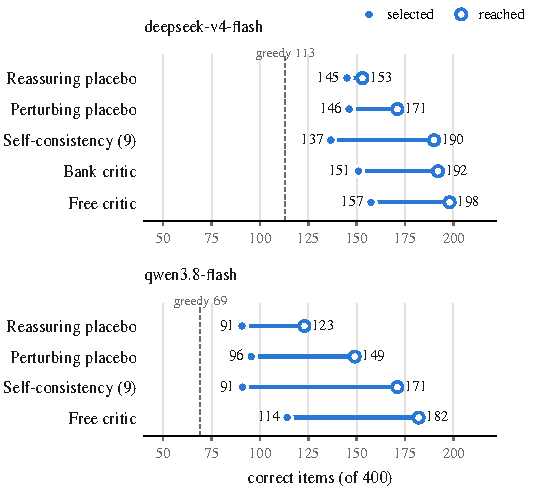
\includegraphics[width=\columnwidth]{figs/reach_select.pdf}
  \caption{Questions out of 400 that each condition \emph{reaches} (the correct answer appears among its answers; open circle) and \emph{selects} (the majority vote over its answers is correct; filled circle), for two models. The free critic reaches about as many questions as nine independent samples and selects the most in every comparison (tests in Table~\ref{tab:pairs}). The dashed line is the greedy first answer that all loops start from.}
  \label{fig:reach}
\end{figure}

On 400 questions of Humanity's Last Exam \citep{phan2025hle} and two models, three results emerge (Figure~\ref{fig:reach}).

\textbf{Critique raises what is reached.}
The number of questions reached rises from the reassuring placebo to the perturbing placebo to the free critic: 153, 171 and 198 on one model, and 123, 149 and 182 on the other.
Both steps are significant on both models.
They remain so when every method is limited to the same number of distinct answers and when only exact matches are counted as correct.

\textbf{Critique also improves what is selected.}
A majority vote over the free critic's answers picks more correct answers than the same vote over either placebo's answers.
The difference is significant on one model and in the pooled data.
The free critic also selects more than a vote over independent samples on both models; on the model where we metered the critic's cost, this holds when sampling is given the same number of tokens.
Restricting the critic to a list of past error types contributes nothing we can identify.

\textbf{The model cannot collect the remainder itself.}
A fifth of the reached questions on one model and more than a third on the other are still not selected.
We asked the same model, in three different ways, to judge its own changes of answer.
Wherever such a judge disagrees with the vote it is right about half of the time, and combining its verdicts with the vote never beats the vote alone on held-out questions.

Our contributions are:
\begin{itemize}
\setlength\itemsep{0pt}
\item a placebo-controlled design that separates the effects of iteration, pressure and critique content, and reports them separately for reaching and for selecting;
\item evidence on two models that specific critique reaches more than the same amount of generic doubt, and that it also improves selection over placebo loops and over sampling at equal cost;
\item two negative results with stated limits: a list of the model's own past error types adds nothing identifiable, and the model's judgements of its own changes of answer add nothing detectable to the vote;
\item all answer sequences, per-round scores, judge verdicts and analysis code.
\end{itemize}

\section{Related Work}

\paragraph{Sampling, coverage and voting.}
Self-consistency returns the most frequent answer among sampled reasoning paths \citep{wang2023selfconsistency}; adaptive variants stop once the vote is settled \citep{aggarwal2023adaptive}, and universal self-consistency lets the model pick the consensus response when answers are free-form \citep{chen2023usc}.
\citet{brown2024monkeys} separate coverage, the fraction of problems solved by any sample, from the ability to identify the solving sample, following the pass@$k$ view of \citet{chen2021codex}, and show that voting plateaus where no verifier exists; gains from more calls can even reverse \citep{chen2024morecalls}, and imperfect verifiers cap what resampling achieves \citep{stroebl2024flaws}.
We apply the same decomposition to trajectories produced by revision.

\paragraph{Self-correction.}
Self-Refine and Reflexion iterate generation and feedback from one model \citep{madaan2023selfrefine,shinn2023reflexion}.
Subsequent studies find that the gains largely vanish without leaked oracle information \citep{huang2024cannot}, that self-critique can hurt where a sound external verifier helps \citep{stechly2024selfverification}, that models locate errors poorly but fix located ones \citep{tyen2024cannot}, and that self-refinement amplifies self-bias \citep{xu2024pride}; \citet{kamoi2024when} survey the conditions under which self-correction works.
\citet{yang2024confidence} decompose accuracy after a correction step into the rate of keeping correct answers and of fixing incorrect ones, an identity we use in Section~\ref{sec:last}.
Closest to our positive result, \citet{bilal2026refining} refine each of several sampled rollouts with self-critique and vote over the refined answers.
A parallel line compares multi-agent debate with voting and attributes most of debate's gains to the vote \citep{smit2024mad,choi2025debate}, and budget-aware evaluation finds that self-consistency often matches or beats reflection and debate at equal compute \citep{wang2024token}.
Pressure without content is known to move answers: challenged with ``Are you sure?'', models flip often and lose accuracy \citep{laban2024flipflop}.
In code repair with execution feedback and small models, placebo-controlled studies find blind resampling hard to beat and disagree on whether feedback content matters beyond a content-free placebo \citep{iscan2026falsification,iscan2026form,verma2026blind}.
Our setting has no executable signal, uses reasoning models on open-domain questions, and separates reaching from selecting.
Our contribution to this line is attribution: the loop is compared against placebos that hold iteration and dose fixed, and effects are reported separately for reaching and for selecting.

\paragraph{Verifiers and judges.}
Trained verifiers supply the external signal that self-correction lacks \citep{lightman2024verify}.
Models used as judges are imperfect and favour their own outputs \citep{zheng2023judging,panickssery2024evaluators}, and consensus among samples is not verification \citep{denisov2026consensus}.
\citet{zhao2025sample} report that same-model verification scales with a large pool of independent responses, and \citet{hu2026oracle} find same-family language-model selectors net negative on fixed pools for mathematics and science questions.
We ask a narrower question: what a model's verdicts on its own changes of answer add once the votes are known.

\section{Setup}
\label{sec:setup}

\paragraph{Loop.}
A solver answers each question greedily (temperature 0, also in later rounds).
In every later round it receives its previous answer and a feedback message and answers again; it is told to keep its answer if it believes the answer is correct.
The loop stops after three identical consecutive answers or after ten feedback rounds.
All loops of a model share the greedy first answer, so they differ only in what follows it.
Solver and critic are the same model, with a reasoning budget of 16{,}384 tokens and 8{,}192 further tokens for visible output per call.

\paragraph{Conditions.}
Table~\ref{tab:conditions} lists the conditions.
The \emph{reassuring placebo} (\rp) returns a fixed sentence stating that no error direction was found.
The \emph{free critic} (\fc) is a separate call to the same model.
It reads the question, the current answer and the end of the solver's reasoning, and must return one to three suspicions, each with a concrete check that the solver can carry out without the reference answer.
It may not name an answer, state a probability or stay silent, and it is told not to re-solve the question.
The \emph{bank critic} (\bc) is identical except that each suspicion must be one of five error archetypes, distilled beforehand from 33 incorrect answers of the same model on six unrelated benchmarks (Appendix~\ref{app:bank}).
The \emph{perturbing placebo} (\pp) calls no model and reads nothing.
It issues suspicions in the critic's output format, built from five fixed generic sentences named after the same archetypes.
The number of suspicions per round is drawn to match what the free critic produces (three in 86\% of rounds), which is what we mean by matching the dose.
\emph{Self-consistency} (\scn) draws nine independent samples at temperature 0.7, and \emph{adaptive self-consistency} consumes them in random order until an answer has three votes.

\begin{table}[t]
\centering
\small
\setlength{\tabcolsep}{3.5pt}
\begin{tabular}{@{}llccc@{}}
\toprule
 & Feedback after round 0 & Iter. & Press. & Content \\
\midrule
\rp & fixed reassuring sentence & \checkmark & & \\
\pp & 1--3 templated suspicions & \checkmark & \checkmark & \\
\bc & 1--3 suspicions, vocabulary & \checkmark & \checkmark & \checkmark \\
\fc & 1--3 suspicions, free & \checkmark & \checkmark & \checkmark \\
\scn & none: 9 samples, $T{=}0.7$ & & & \\
\bottomrule
\end{tabular}
\caption{Conditions and the respects in which they differ: iteration over one's own answer, pressure on it, and feedback content generated for the question and answer. \rp: reassuring placebo; \pp: perturbing placebo; \bc: bank critic; \fc: free critic; \scn: self-consistency.}
\label{tab:conditions}
\end{table}

\paragraph{Models and data.}
We use 400 text-only questions of Humanity's Last Exam, sampled with stratification by subject category (84 multiple choice, 316 open-form).
The main experiment uses deepseek-v4-flash (\ds) for all conditions.
A replication on the same questions uses qwen3.8-flash (\qw) for all conditions except the bank critic, whose vocabulary was distilled for the first model.
Trajectories in which any call failed at the interface were discarded and rerun in full.

\paragraph{Scoring.}
Every answer of every round is scored once.
Answers are compared with the reference by exact matching after type-specific normalization; unmatched answers are judged by an independent model from a different provider; disputed answer variants are adjudicated under the rule that the same substance receives the same verdict in every condition and round (Appendix~\ref{app:scoring}).
A round truncated at the token limit is scored as incorrect.
Because the model-based tier can only add acceptances, we repeat the main comparisons with exact matching alone.

\paragraph{Reaching and selecting.}
We call the sequence of answers a loop produces its \emph{trajectory}, and the distinct answers in a trajectory or in a set of samples its \emph{candidates}; two answers are the same candidate if they agree after normalization (option letter, integer, or normalized string).
A question is \emph{reached} if some candidate is correct, and \emph{reach} is the number of questions reached.
A question is \emph{selected} if the most frequent candidate is correct: the \emph{mode} over the rounds of a loop, or the \emph{vote} over samples.
We also report the \emph{final} answer of each loop.
When several candidates tie for the most votes, we break the tie at random in every condition and score the question by its expected value, for example 0.5 when one of two tied candidates is correct.
A loop could instead prefer its most recent answer, but independent samples have no order, so that rule would favour loops.

\paragraph{Statistics.}
Conditions are compared on the same questions.
Binary outcomes (reached, final answer) use exact McNemar tests, reported with discordant counts.
Selected answers use a paired sign-flip permutation test on per-question expected scores (10{,}000 permutations) with 95\% bootstrap intervals over questions.
For pooled tests we add the two models' differences on each question, since both models answer the same questions.
$P$-values are unadjusted.
Appendix~\ref{app:prereg} states which analyses were specified before their data were seen: the comparison with self-consistency, the contrast in reach between the free critic and the perturbing placebo, the vocabulary contrast, the acceptance criteria for judges, the four replication tests and the cost-matched comparisons.
Selection contrasts against the placebos, pooled tests, and the candidate-matched and exact-match reachs are exploratory.

\section{Results}

\begin{table*}[t]
\centering
\small
\setlength{\tabcolsep}{4.2pt}
\begin{tabular}{@{}l rrrrr c rrrrr@{}}
\toprule
 & \multicolumn{5}{c}{\ds{} (greedy 113)} & & \multicolumn{5}{c}{\qw{} (greedy 69)} \\
\cmidrule(lr){2-6}\cmidrule(l){8-12}
Condition & Final & Selected & Reached & Cand. & Tokens & & Final & Selected & Reached & Cand. & Tokens \\
\midrule
Reassuring placebo & 141 & 145.0 & 153 & 2.1 & 24.6 & & 89 & 90.8 & 123 & 2.1 & 15.2 \\
Perturbing placebo & 142 & 146.1 & 171 & 2.7 & 31.8 & & 92 & 95.6 & 149 & 2.9 & 21.0 \\
Self-consistency, 9 samples & -- & 136.7 & 190 & 4.5 & 51.4 & & -- & 91.0 & 171 & 4.8 & 31.8 \\
Self-consistency, 11 samples & -- & 138.2 & 193 & -- & 61.8 & & -- & -- & -- & -- & -- \\
Adaptive self-consistency & -- & 135.8 & -- & -- & 35.5 & & -- & -- & -- & -- & -- \\
Bank critic & 140 & 150.9 & 192 & 3.5 & 66$^{\ast}$ & & -- & -- & -- & -- & -- \\
Free critic & \textbf{148} & \textbf{157.4} & \textbf{198} & 3.7 & 61$^{\ast}$ & & \textbf{112} & \textbf{114.1} & \textbf{182} & 3.6 & 23.6$^{\dagger}$ \\
\bottomrule
\end{tabular}
\caption{Correct questions out of 400. \emph{Final}: last answer of the loop. \emph{Selected}: mode over rounds or vote over samples, expected score under random ties. \emph{Reached}: some candidate is correct. \emph{Cand.}: distinct candidates per question. \emph{Tokens}: millions, prompt plus completion. $^{\ast}$Includes critic calls, estimated at 23 (free) and 29 (bank) million from a replay of 50 calls per critic. $^{\dagger}$Solver only; critic calls were not metered for this model.}
\label{tab:main}
\end{table*}

Table~\ref{tab:main} gives the main results and Table~\ref{tab:pairs} the paired comparisons.

\subsection{Critique raises what is reached}
\label{sec:reach}

On both models reach rises across the three loops.
The perturbing placebo reaches more questions than the reassuring placebo (\ds{} 171 against 153, \qw{} 149 against 123), and the free critic reaches more than the perturbing placebo (198 against 171, 182 against 149).
All four differences are significant (Table~\ref{tab:pairs}).
The free critic reaches about as many questions as nine independent samples (198 against 190 and 182 against 171; $p=0.32$ and $0.25$) while producing fewer candidates per question.

A method that produces more candidates has more chances to hit the correct answer, and the conditions differ in how many they produce (Table~\ref{tab:main}).
The gap between the free critic and the perturbing placebo could therefore reflect quantity alone.
Table~\ref{tab:robust} rules this out by counting only the first $k$ candidates of each trajectory.
The free critic stays ahead of the perturbing placebo at $k=2$ and $k=3$ on both models (\ds{} discordant pairs 33/9 and 35/11, $p\le 0.001$; \qw{} 37/19 and 41/18, $p=0.02$ and $0.004$).
The difference is already present at the first change of answer: on \ds{}, when the first candidate is wrong and the loop moves to a second one, that second candidate is correct 24\% of the time under the free critic (48 of 204) and 15\% under the perturbing placebo (26 of 171).

Table~\ref{tab:robust} also addresses the scorer.
The model-based scoring tier can only accept additional answers, so it could favour conditions with more candidates.
When only exact matches count, every number falls and the order of the three loops is unchanged (free critic against perturbing placebo: 31/11, $p=0.003$, and 35/12, $p=0.001$).
One comparison does depend on the scorer: on \qw{} the free critic and self-consistency reach similar numbers under full scoring (182 and 171) but not under exact matching (117 and 93).

\begin{table}[t]
\centering
\small
\setlength{\tabcolsep}{3.2pt}
\begin{tabular}{@{}l rrrr c rrrr@{}}
\toprule
 & \multicolumn{4}{c}{\ds} & & \multicolumn{4}{c}{\qw} \\
\cmidrule(lr){2-5}\cmidrule(l){7-10}
 & \rp & \pp & \scn & \fc & & \rp & \pp & \scn & \fc \\
\midrule
First 2 cand. & 141 & 148 & 169 & 172 & & 109 & 118 & 134 & 136 \\
First 3 cand. & 150 & 157 & 178 & 181 & & 118 & 137 & 147 & 160 \\
All cand. & 153 & 171 & 190 & 198 & & 123 & 149 & 171 & 182 \\
Exact match & 91 & 102 & 120 & 122 & & 79 & 94 & 93 & 117 \\
\bottomrule
\end{tabular}
\caption{Robustness of reach: questions reached within the first $k$ candidates, and with exact-match scoring only (all candidates). Abbreviations as in Table~\ref{tab:conditions}.}
\label{tab:robust}
\end{table}

\begin{table*}[t]
\centering
\small
\setlength{\tabcolsep}{4.5pt}
\begin{tabular}{@{}l lll c lll@{}}
\toprule
 & \multicolumn{3}{c}{\ds} & & \multicolumn{3}{c}{\qw} \\
\cmidrule(lr){2-4}\cmidrule(l){6-8}
Comparison & Reached & Selected, $\Delta$ [95\% CI] & $p$ & & Reached & Selected, $\Delta$ [95\% CI] & $p$ \\
\midrule
\fc{} vs \rp & 52/7$^{***}$ & $+12.4$ \ci{-1.6}{25.6} & .08 & & 69/10$^{***}$ & $+23.3$ \ci{8.8}{39.2} & .004 \\
\fc{} vs \pp & 39/12$^{***}$ & $+11.3$ \ci{-0.8}{23.7} & .07 & & 49/16$^{***}$ & $+18.5$ \ci{3.9}{34.3} & .02 \\
\pp{} vs \rp & 28/10$^{**}$ & $+1.2$ \ci{-10.1}{12.5} & .84 & & 42/16$^{***}$ & $+4.8$ \ci{-8.1}{18.6} & .47 \\
\fc{} vs \scn{} (9) & 29/21 & $+20.7$ \ci{9.0}{32.4} & $<$.001 & & 44/33 & $+23.1$ \ci{9.6}{38.6} & .002 \\
\fc{} vs \scn{} (11) & -- & $+19.2$ \ci{7.0}{31.1} & .002 & & -- & -- & -- \\
\rp{} vs \scn{} (9) & 9/46$^{***}$ & $+8.2$ \ci{-4.0}{21.1} & .20 & & 11/59$^{***}$ & $-0.2$ \ci{-12.9}{12.1} & .99 \\
\fc{} vs \bc & 23/17 & $+6.5$ \ci{-6.4}{18.9} & .32 & & -- & -- & -- \\
\bc{} vs \scn{} (9) & 24/22 & $+14.1$ \ci{2.5}{26.7} & .03 & & -- & -- & -- \\
\bc{} vs \rp & 47/8$^{***}$ & $+5.9$ \ci{-6.8}{18.5} & .34 & & -- & -- & -- \\
\bc{} vs \pp & 36/15$^{**}$ & $+4.8$ \ci{-6.5}{16.4} & .43 & & -- & -- & -- \\
\bottomrule
\end{tabular}
\caption{Paired comparisons on 400 questions. \emph{Reached}: discordant questions (first condition only / second only), exact McNemar, $^{**}p<0.01$, $^{***}p<0.001$. \emph{Selected}: difference in expected score, bootstrap interval, permutation test. Abbreviations as in Table~\ref{tab:conditions}; the number of samples is in parentheses.}
\label{tab:pairs}
\end{table*}

\subsection{Critique improves what is selected}
\label{sec:select}

\paragraph{Against placebo loops.}
Here both methods are loops and both are scored by the same vote, so the only difference is the feedback (Figure~\ref{fig:forest}).
On \qw{} the free critic selects 23.3 more correct answers than the reassuring placebo and 18.5 more than the perturbing placebo, both significant.
On \ds{} the differences are 12.4 and 11.3, with intervals that reach zero.
Pooled over the two models, the mean difference per model is 17.9 against the reassuring placebo (\ci{7.8}{28.5}, $p<0.001$) and 14.9 against the perturbing placebo (\ci{5.3}{25.7}, $p=0.003$).

Three cautions apply.
These comparisons were not among the tests we specified in advance.
The bank critic, for which the study was first designed, exceeds the placebos by only 5.9 and 4.8 on \ds{} (Table~\ref{tab:pairs}), and the difference between the two models is not itself significant ($10.8$, \ci{-8.8}{31.6}).
And the critic call roughly doubles the computation of the loop.
We therefore regard the selection gain over placebo loops as supported on one model and suggestive overall.

Pressure alone yields no detectable selection gain on either model ($+1.2$ and $+4.8$): the perturbing placebo adds candidates, but the vote does not turn them into correct selections.

\begin{figure}[t]
  \centering
  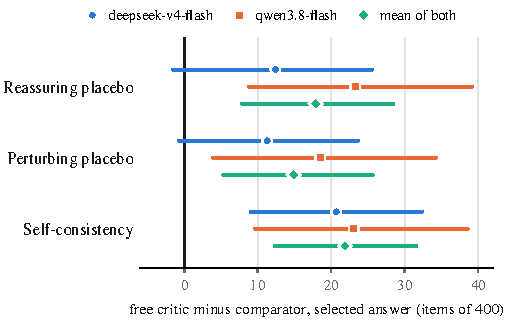
\includegraphics[width=\columnwidth]{figs/forest.pdf}
  \caption{Difference in selected correct answers between the free critic and each comparator, with 95\% bootstrap intervals. Self-consistency uses nine samples; at matched cost (eleven samples) the difference on deepseek-v4-flash is 19.2.}
  \label{fig:forest}
\end{figure}

\paragraph{Against self-consistency.}
The free critic selects more correct answers than nine-sample self-consistency on both models ($+20.7$ and $+23.1$).
On \ds{} the critic's total token use corresponds to eleven samples; with two further samples self-consistency rises from 136.7 to 138.2 and the difference remains ($+19.2$, \ci{7.0}{31.1}, $p=0.002$).
The reassuring placebo matches self-consistency with about half its tokens on both models and does not exceed it significantly.
Sampling is not handicapped by its temperature: a single sample is correct on 117 and 80 questions on average, against 113 and 69 for the greedy answer.

Two analyses qualify the margin over self-consistency.

The first concerns how answers are written.
The gain is confined to open-form questions, where independent samples may write the same answer in different ways and so split their vote.
Stripping formatting before voting changes nothing (\ds{} $+21.6$).
To bound how much splitting could matter, we give sampling the benefit of the doubt: before voting we treat all answers to a question that were scored correct as one candidate, in every condition.
This needs the reference answers, so it is a diagnostic and not a usable method, and it also merges answers that differ in substance, so it overstates the effect.
Under this bound the free critic's margin over nine samples is $+13.0$ on \ds{} (\ci{2.1}{23.8}) and $+12.2$ on \qw{} (\ci{-2.8}{27.3}), or 12.6 per model pooled (\ci{3.2}{22.4}, $p=0.010$); over eleven samples on \ds{} it is $+9.3$ (\ci{-2.1}{20.4}).
The margin over placebo loops is unaffected (pooled $p<0.001$).

The second is universal self-consistency, in which the model itself is asked to pick the consensus among the samples.
On the 396 \ds{} questions whose samples were not rerun, it selects 145 from eleven samples where the plain vote selects 138, and the free critic's mode exceeds it by 11.4 (\ci{-1.4}{24.8}, $p=0.09$).
We had decided beforehand that a failure of this test would limit the claim, and it does.
The free critic beats the standard vote at equal cost; we cannot claim that it beats sampling once equivalent answers are merged, whether by the bound above or by a model-based selector.
Applied to the critic's own rounds, that selector does not improve on the mode (153 against 157).

\paragraph{The vocabulary.}
The free critic is at least as good as the bank critic on every measure and the differences are not significant (Table~\ref{tab:pairs}).
We had specified that the vocabulary would count as not identifiable if the free critic's reach fell no more than five questions below the bank critic's; it is six questions above.
This five-archetype vocabulary therefore adds nothing we can detect to a critic that is free to name the shortcoming itself; the two critics also differ in how many suspicions they issue (Appendix~\ref{app:prompts}).

\paragraph{What the controls do not isolate.}
The free critic differs from the perturbing placebo in three ways: it reads the question, it reads the answer, and it is produced by a model call with its own reasoning budget.
A critic could therefore help simply by solving the problem again and passing its solution on.
We checked for this on the changes of answer that turn a wrong answer into a correct one or the reverse.
If the critic were handing over solutions, its text should contain the solver's next answer, and mainly when the change is for the better.
It rarely does (\ds{} 2 of 132 changes for the better with a numeric or free-text answer, \qw{} 17 of 159), and no more often than for changes for the worse (2 of 100 and 16 of 132).
Changes for the better and for the worse are also about equally common (165 and 135; 229 and 193).
This check cannot detect a critic that gives a derivation and stops short of the answer.
A critic that reads the question but not the answer, and a control matched in tokens, would settle the matter; we leave them to future work and attribute the effects to specific critique of the question and answer.

\subsection{The last-answer benefit is significant on one model}
\label{sec:last}

On \ds{} the last answer of the free critic is no better than that of the reassuring placebo (148 against 141; discordant 29/22, $p=0.40$), in line with the negative literature.
On \qw{} it is better (112 against 89; 48/25, $p=0.010$, and 41/21 against the perturbing placebo, $p=0.015$), although the difference between the two models is not itself significant ($16.0$, \ci{-4.0}{38.0}).
A simple accounting identity \citep{yang2024confidence} shows why the starting accuracy matters.
One round of revision fixes some wrong answers and breaks some correct ones.
It raises accuracy only if the fraction of wrong answers fixed, divided by the fraction of correct answers broken, exceeds $a/(1-a)$, where $a$ is the accuracy before revision.
That bar is 0.39 on \ds{} ($a=0.28$) and 0.21 on \qw{} ($a=0.17$), and every loop clears it on both models (first-round ratios between 0.34 and 0.96).
At a starting accuracy of 0.8 the bar is 4, and the same loops would lower accuracy; most negative results were obtained on tasks where models start that high.
In every loop the mode is at least as good as the last answer (Table~\ref{tab:main}), so a loop is better judged by all of its answers than by its last.

\subsection{Why the count works}
\label{sec:mech}

The vote selects correct answers because a correct answer is more likely to be repeated than an incorrect one.
Table~\ref{tab:stay} gives the probability that the next answer repeats the current one.
In every condition correct answers are repeated more often than incorrect ones, and the ratio is highest under the free critic on both models.
On \qw{} the lower bound of its interval (1.37) exceeds the reassuring placebo's estimate (1.20), which was the criterion we had set for the replication.
Under reassurance all answers tend to be kept; under critique incorrect answers are dropped more readily than correct ones; independent samples agree least.

Two cautions apply.
Loops stop after three repeats, so repeating an answer and winning the vote are linked by design.
And for sampling the table reports how often two samples agree, which is a different quantity.
The table describes the conditions and does not by itself explain the margin over sampling.
The vote also undercounts correct answers: on \ds{}, 27\% of the steps from one correct answer to another under the critics change how the answer is written (16\% under reassurance).

\begin{table}[t]
\centering
\small
\setlength{\tabcolsep}{3.6pt}
\begin{tabular}{@{}l ccc c ccc@{}}
\toprule
 & \multicolumn{3}{c}{\ds} & & \multicolumn{3}{c}{\qw} \\
\cmidrule(lr){2-4}\cmidrule(l){6-8}
 & corr. & inc. & ratio & & corr. & inc. & ratio \\
\midrule
\rp & .77 & .54 & 1.4 & & .68 & .56 & 1.2 \\
\pp & .69 & .41 & 1.7 & & .51 & .40 & 1.3 \\
\scn & .50 & .28 & 1.8 & & .36 & .26 & 1.4 \\
\bc & .52 & .30 & 1.7 & & -- & -- & -- \\
\fc & .53 & .25 & \textbf{2.1} & & .46 & .29 & \textbf{1.6} \\
\bottomrule
\end{tabular}
\caption{Probability that the next answer repeats the current one, for correct and incorrect current answers (self-consistency: over ordered pairs of samples), and their ratio. Bootstrap intervals for the ratios are in Appendix~\ref{app:more}.}
\label{tab:stay}
\end{table}

\section{Can the Model Collect the Remainder?}
\label{sec:judges}

On \ds{} the bank critic reaches 191 questions and its mode with a recency tie rule selects 154.\footnote{This analysis uses the bank critic's trajectories as first recorded; three were later rerun after interface failures, which moves reach to 192 in Table~\ref{tab:main}; the mode here uses the recency tie rule (154, against 150.9 under random ties).}
We ask whether the same model can recover any of the remaining 37 by judging the loop's own changes of answer.

\paragraph{Headroom.}
Of the 37 questions, 11 are ties, 10 are lost by one vote and 16 by more.
We call a change from one answer to a different one in consecutive rounds a \emph{switch}.
The trajectories contain 1{,}201 switches, of which 159 turn an incorrect answer into a correct one and 142 do the opposite.
An oracle that undoes every harmful switch reaches 173 selected questions.
Undoing every switch that the solver attributes to the feedback, good or bad, gives 149, worse than the mode.
Recovery therefore requires telling good switches from bad ones.

\paragraph{Judges and aggregation.}
We test three framings with the same model and no reference answers.
\emph{Judge-R} scores the new answer of a switch on three rubric dimensions.
\emph{Judge-R+} additionally sees the question and must quote the step it objects to.
\emph{Judge-C} judges the critique instead: whether the suspicion that preceded the switch was warranted.
To use the verdicts, we let them adjust the vote.
Each candidate's vote count is raised or lowered according to the verdicts on the switches into and out of it, weighted by how reliable each kind of verdict has proved to be (a likelihood ratio, added in log space).
Reliability is estimated on half of the questions and applied to the other half, in both directions.
If the verdicts carry no information, the rule returns the plain mode.

\begin{table}[t]
\centering
\small
\setlength{\tabcolsep}{3.5pt}
\begin{tabular}{@{}l ccc@{}}
\toprule
 & Judge-R & Judge-R+ & Judge-C \\
\midrule
Switches judged & 1{,}185 & 1{,}041 & 1{,}201 \\
Acc., decisive switches & .58 & .60 & .66 \\
Fit dev, apply test (76) & 76 & 73 & 71 \\
Fit test, apply dev (78) & 73 & 72 & 77 \\
Acc.\ where it disagrees & 18/36 & 53/116 & 32/66 \\
\quad with the votes & (.50) & (.46) & (.49) \\
Best of 81 rules, in-sample & 154 & 156 & 155 \\
\bottomrule
\end{tabular}
\caption{Same-model judges on the bank critic's trajectories (\ds). Decisive switches change correctness. The mode selects 76 and 78 correct questions on the two halves and 154 overall.}
\label{tab:judges}
\end{table}

\paragraph{Results.}
No judge improves on the mode in either direction of the split (Table~\ref{tab:judges}).
Two of the three judges are better than chance at telling whether a single switch was an improvement.
But so is a rule that ignores the judge and looks only at the votes: guess that a switch was an improvement if the new answer ends up with at least as many votes as the old one.
The judges are no more accurate than this rule.
A judge can change the outcome only where it disagrees with the rule, and there its accuracy is 0.50, 0.46 and 0.49, with every interval containing one half.
A sweep over 81 ways of combining verdicts and votes gains at most two questions in-sample and none when the best rule on one half is applied to the other.

Why is 66\% accuracy on single switches not enough?
Overturning the mode helps on only 37 of the 123 questions where it is possible (30\%).
At that base rate, a judge that is right with probability $p$ overturns correctly with probability $0.30p/(0.30p+0.70(1-p))$, which exceeds one half only when $p>0.70$.

In short, once the votes are known, none of the three judges told us anything more about which answer was correct.
The statement covers one model and the trajectories of one condition and has the resolution of 400 questions: with 36 to 116 disagreements per judge, accuracies of up to about 0.65 are not excluded.
It does not conflict with verification over large pools of independent responses \citep{zhao2025sample}: our judges see one trajectory of three to four candidates, produced by a solver that has already responded to critique from the same model.

\section{Discussion}

\paragraph{Two gains, three sources.}
Iterating and voting is cheap, and it selects as well as self-consistency with half the tokens.
Pressure adds reach and no detectable selection gain.
Specific critique adds more reach and, on our evidence, selection as well: 12 questions on one model, not significant on its own, and 23 on the other.
On both models the critic gains less in selection than in reach, because every new answer it provokes also competes in the vote, and the vote can only favour answers that come back.

\paragraph{Reconciling the two readings.}
Whether a study finds self-critique helpful depends on what it compares and what it scores.
Against sampling, a loop looks good partly because it iterates.
Against a placebo loop, the benefit of critique is smaller and still present.
Scored by the last answer, the benefit can vanish on a model that starts at higher accuracy.

\paragraph{Cost and use.}
On \ds{} the free critic uses 2.5 times the tokens of the reassuring placebo and 1.2 times those of nine-sample self-consistency.
Where nothing can verify an answer, that extra cost buys roughly 12 to 23 selected questions.
Where answers can be verified by something other than the model, what matters is reach: there the critic exceeds the placebo loop by 45 and 59 questions and matches or exceeds sampling with fewer candidates.

\section{Conclusion}

A self-critique loop gains in what it reaches and in what it selects.
On two models, placebo controls show that specific critique reaches more than iteration alone and more than the same amount of generic doubt, and they indicate that it also improves what is selected, significantly on one model and in the pooled data.
A list of the model's own past error types adds nothing identifiable, and the model's judgements of its own changes of answer add nothing detectable to the vote.
Between a fifth and more than a third of what critique reaches remains unselected, and none of the same-model selectors we tried recovered it.

\section*{Limitations}

The study uses two models from the same price tier and one benchmark, with one run per condition, and no role was tuned.
The benchmark's reference answers are known to contain errors \citep{zhai2026hleverified}, which adds noise to every condition.

The selection advantage over placebo loops was not among the pre-specified tests; it is significant on one model and in the pooled data, and the bank critic does not show it.
The margin over self-consistency depends on how equivalent answers are treated; it is not established against universal self-consistency, which we ran on one model only.
The original falsification test was written for the bank critic, which passes it ($p=0.03$); the free critic was introduced afterwards as a control.

The perturbing placebo controls for pressure, dose and format, and not for generation, length, reading the question, or the additional computation of the critic call; its dose distribution was taken from the first model and reused for the second.
We therefore attribute the effects to specific critique and not specifically to reading the answer.

Critic token counts are extrapolated from a replay on one model and were not metered on the other, and we did not tune the critic's reasoning budget for cost.

Free-form answers are scored by a protocol whose model-based tier has not been audited by human annotators; the results on reach hold under exact matching alone.
For the replication and for added samples the adjudication rules of the main experiment were reused without a new round of dispute resolution, uniformly across conditions.
Conditions of the main experiment were served through two endpoints of the same model weights; reasoning length and truncation rates agree across them.

The judge study covers one model and one condition.
Pre-specification was recorded in dated internal documents and not registered externally, and $p$-values are unadjusted for the number of comparisons.

\section*{Ethics Statement}

The study uses a public benchmark and commercial model interfaces and involves no human subjects.
Its results concern the reliability of model self-evaluation; we see no specific risk beyond those of the underlying models.

\bibliography{refs}

\appendix

\section{Conditions and Prompts}
\label{app:prompts}

\paragraph{Solver.}
Round 0 uses the benchmark prompt.
In later rounds the solver receives the question again together with this message: ``A reviewer looked at your PREVIOUS answer to this question and gave feedback. Your previous answer was: [answer]. Reviewer feedback: [feedback]. Reconsider the question and provide your final answer again. If you believe your previous answer was already correct, keep it as is.''
Each round is an independent call; no conversation history is carried.

\paragraph{Reassuring placebo.}
The feedback is the fixed sentence ``No confident error direction was found for this answer.''

\paragraph{Critics.}
The critic's system prompt states that it inspects a committed answer to a hard question and identifies the most likely wrong directions; that it never reads the reference answer, never emits a probability, never names the correct answer or any answer content, and speaks only of possibilities.
The user message contains the question, the answer, and the last 6{,}000 characters of the solver's reasoning.
The critic returns one to three objects, each with a short label, a suspicion grounded in this answer's specific shortcoming, and a concrete check that the solver can run without the reference answer; it is told not to re-derive or re-solve the question.
The bank critic's prompt differs in four places: the system prompt refers to a supplied vocabulary instead of the critic's own judgement; the user message lists the five archetypes with their definitions and check procedures; the label must be an archetype name; and when the critic fails after one retry, the bank critic falls back to a retrieved archetype whereas the free critic falls back to the reassuring sentence (30 of 2{,}358 rounds on \ds).
On \ds{} the free critic returned three suspicions in 86\% of rounds; the bank critic returned one in 57\% and three in 12\%.
On \qw{} the free critic returned three in 95\% of rounds.

\paragraph{Perturbing placebo.}
Each round draws $k\in\{3,2,1\}$ with probabilities 0.86, 0.11 and 0.03 and then $k$ of the five archetypes without replacement, seeded by the question identifier and the round; the same distribution was used for both models.
Each is rendered as ``[name]: you may have [generic suspicion]. To check: [generic check].'', for example ``constraint-blind decimation: you may have discounted a constraint or condition stated in the problem. To check: re-read the problem statement, list every stated constraint, and confirm the answer satisfies each one.''
No model is called.

\paragraph{Self-consistency.}
Samples use the round-0 prompt at temperature 0.7.
The adaptive variant is simulated on the recorded samples over 200 random orders.

\section{Error Vocabulary}
\label{app:bank}

The vocabulary was distilled from 33 incorrect single-shot answers of deepseek-v4-flash on GPQA-Diamond, MMLU-Pro, MATH-500, BFCL, BBH and AIME.
Each error was abstracted into an answer-free description of the faulty operation and a check procedure, and the descriptions were merged across benchmarks into five archetypes: constraint-blind decimation; descriptor or label conflation; procedure truncation or omission; retrieval abort; format or precision non-conformance.
No question, answer or error from Humanity's Last Exam enters the vocabulary, and no entry contains a reference answer.

\section{Scoring Protocol}
\label{app:scoring}

\paragraph{Tiers.}
(1) A round whose generation was truncated at the token limit is incorrect.
(2) Otherwise the answer is matched against the reference by type-specific rules (option letter, integer, normalized string).
(3) Unmatched answers are judged once by a model from a different provider (gpt-6-astra), with the verdict cached per question and answer so that identical answers receive identical verdicts in all conditions.
(4) For the main experiment, answers on which this judge and a second model-based check disagreed were re-judged three times and adjudicated per answer variant; the resulting rules are applied wherever the same variant recurs.
For the replication and for the two added self-consistency samples, tiers (1) to (3) and the existing rules of tier (4) were applied.

\paragraph{Selection rules.}
A candidate is correct if its last occurrence is scored correct.
A truncated round may contribute a vote when an answer can be recovered from the end of its reasoning, but a truncated winner is incorrect.
The recency tie rule for loops, which returns the tied answer that occurred last, was fixed in the scoring code before any comparison; it gives 144, 147, 154 and 159 for the reassuring placebo, perturbing placebo, bank critic and free critic on \ds{}, against 145.0, 146.1, 150.9 and 157.4 under random ties.

\paragraph{Interface failures.}
Any trajectory containing a failed call was rerun in full: 29 questions for the perturbing placebo, between one and four for the other conditions of the main experiment, and 61 first answers with their dependent trajectories in the replication.
An error message never counts as an answer.

\paragraph{Truncation.}
On \ds{} between 6.4\% and 8.0\% of rounds per condition are truncated at the token limit, including 28 of the 400 greedy first answers; on \qw{} one round is truncated.

\section{Pre-Specified Analyses}
\label{app:prereg}

The following were written down, with dates, before the corresponding data were seen.
(i) The falsification test: the mode of the critic loop against nine-sample self-consistency on paired questions; written for the bank critic.
(ii) The reassuring placebo as the control for iteration (no outcome threshold was fixed).
(iii) The read-out for the free critic: the vocabulary is ``not identifiable'' if the free critic's reach is no more than five questions below the bank critic's and their persistence intervals overlap.
(iv) The read-out for the perturbing placebo: content is ``effective'' if the placebo's reach is at least 15 questions below the free critic's at $p<0.05$ (observed: 27 below on \ds, 33 below on \qw).
(v) Acceptance criteria for judges: accuracy on decisive switches, intervals of likelihood ratios, the split-half comparison with the mode, and stability across halves.
(vi) Replication tests on the second model: free critic against self-consistency on the selected answer; reach of the free critic against the reassuring placebo; persistence ratio of the free critic above that of the reassuring placebo; reach of the perturbing placebo against the free critic.
All four hold.
(vii) Cost-matched comparisons on the first model: free critic's mode against the vote over eleven samples (holds) and against universal self-consistency over eleven samples (interval includes zero), with the rule that failure of the second qualifies the selection claim.

The reach--select decomposition as applied here, the selection contrasts against the placebos, the contrast between the two placebos, the break-even criterion, the candidate-matched and exact-match reachs, the pooling bound, the pooled two-model tests, selective prediction and the verifier simulation are exploratory.
The random-tie convention replaced an earlier asymmetric one after internal review.

\section{Additional Results}
\label{app:more}

\paragraph{Persistence intervals.}
Bootstrap 95\% intervals of the ratios in Table~\ref{tab:stay}: \ds{} \rp{} \ci{1.27}{1.58}, \pp{} \ci{1.50}{1.88}, \scn{} \ci{1.45}{2.14}, \bc{} \ci{1.50}{2.01}, \fc{} \ci{1.83}{2.50}; \qw{} \rp{} \ci{1.07}{1.34}, \pp{} \ci{1.12}{1.43}, \scn{} \ci{1.10}{1.70}, \fc{} \ci{1.37}{1.83}.

\paragraph{First-round repair and damage.}
Questions repaired and damaged by the first revision: \ds{} \rp{} 17 and 7, \pp{} 22 and 13, \bc{} 38 and 19, \fc{} 45 and 20; \qw{} \rp{} 30 and 13, \pp{} 40 and 18, \fc{} 47 and 29.

\paragraph{Universal self-consistency.}
The selector is the solver model at temperature 0 with the prompt of \citet{chen2023usc}, given the final answers of an question in random order.
Unparseable outputs (1.3\% to 4.5\% per condition) fall back to the vote.
On the 396 questions whose samples were not rerun it selects 142 from nine samples and 145 from eleven (vote on the same questions: 138), at about 5{,}000 reasoning tokens per call.
Applied to loop trajectories it selects 153 for the free critic, 151 for the bank critic and 144 for the reassuring placebo.

\paragraph{Pooling bound.}
Selected answers when all answers of an question that were scored correct are pooled into one candidate: \ds{} \rp{} 145.5, \pp{} 149.1, \scn{} 149.8 (153.6 with eleven samples), \bc{} 159.9, \fc{} 162.9; \qw{} \rp{} 92.5, \pp{} 101.1, \scn{} 104.6, \fc{} 116.8.
Free critic against reassuring placebo under the bound: \ds{} $+17.4$ \ci{3.6}{30.3}, \qw{} $+24.2$ \ci{9.2}{40.4}.
Free critic against eleven-sample self-consistency under the bound (\ds): $+9.3$ \ci{-2.1}{20.4}, $p=0.11$.

\paragraph{Differences between models.}
Difference of differences, \qw{} minus \ds{}, on the shared questions: free critic against reassuring placebo, selected $+10.8$ \ci{-8.8}{31.6} and final $+16.0$ \ci{-4.0}{38.0}; against perturbing placebo, selected $+7.2$ \ci{-10.6}{26.7}; against self-consistency, selected $+2.4$ \ci{-15.5}{20.9}.

\paragraph{Abstention.}
Ranking questions by the margin between the two most frequent answers and answering only the most confident fraction gives, on \ds{}, accuracies at coverage 1.0, 0.8, 0.5 and 0.33 of .360, .391, .425, .386 for the reassuring placebo; .342, .386, .445, .470 for self-consistency; .385, .425, .485, .515 for the bank critic; and .398, .453, .510, .492 for the free critic.
The area under the ROC curve of the margin is 0.59, 0.64, 0.64 and 0.64.

\paragraph{Imperfect external verification.}
We simulate a verifier that accepts each candidate independently with accuracy $q$ and return the most frequent accepted candidate, falling back to the mode.
On \ds{} at $q=0.7$ and $0.9$ the simulated correct counts are 143 and 150 for the reassuring placebo, 152 and 177 for self-consistency, 161 and 181 for the bank critic, and 166 and 187 for the free critic.
When verifier accuracy is assumed to fall with the number of candidates and on questions the greedy answer got wrong, the counts at $q=0.7$ are 140, 135, 147 and 154.

\paragraph{Other selection rules.}
\emph{Settle} returns the answer of the last run of at least three identical answers and is incorrect when no such run exists; on \ds{} it gives 135, 134, 117 and 121 for the reassuring placebo, perturbing placebo, bank critic and free critic.

\section{Judge Details}
\label{app:judges}

Judge-R assigns scores to three dimensions of the new answer (disconnection from established steps, contradiction, a locatable error) and votes to cut the answer when any score is high.
Judge-R+ adds the question, a required quotation of the step objected to, and a class of falsifier; it covers 1{,}041 of the 1{,}201 switches, and Judge-R returned a verdict on 1{,}185.
Judge-C receives the question, the suspicion and the criticized answer and decides whether the suspicion was warranted; a verdict requires agreement across two presentations in swapped order.
Likelihood ratios with intervals that exclude one were obtained for Judge-R+ (cut 0.72, keep 1.90) and Judge-C (unwarranted 0.51, warranted 1.87), and not for Judge-R.
The 81 aggregation rules vary where a verdict acts (the boundary round, the run, or the whole candidate), the weights of the two verdict directions, and gating to low-margin questions.
On the 56 tied questions Judge-C is right on 17 of 26 disagreements ($p=0.17$), and the recency rule alone recovers 14 of the 23 ties whose tied set contains the correct answer.
A contrast of 26 reference-free trajectory features between repairing and damaging switches gives areas under the curve between 0.43 and 0.59, none stable across halves.

\end{document}
